%% main.tex — G4: Multi-Substation WAPC Scaling
%% IEEE Transactions on Smart Grid
%% Target: 7 pages, submitted 2026-04
%% Author: Anoop V. Eluvathingal, IIT Madras
%% ============================================================
\documentclass[journal]{IEEEtran}

%% ── Fonts & encoding ─────────────────────────────────────────────────────────
\usepackage[T1]{fontenc}
\usepackage[utf8]{inputenc}
\usepackage{microtype}

%% ── Maths ────────────────────────────────────────────────────────────────────
\usepackage{amsmath,amssymb,amsthm,bm}

%% ── Tables ───────────────────────────────────────────────────────────────────
\usepackage{booktabs,array,multirow,tabularx}

%% ── Graphics & TikZ ──────────────────────────────────────────────────────────
\usepackage{graphicx}
\usepackage{tikz}
\usetikzlibrary{arrows.meta,shapes.geometric,positioning,calc,patterns,
                decorations.pathmorphing,decorations.pathreplacing}
\usepackage{pgfplots}
\pgfplotsset{compat=1.18}

%% ── Miscellaneous ────────────────────────────────────────────────────────────
\usepackage{cite}
\usepackage{url}
\usepackage{enumerate}

%% ── Theorem environments ─────────────────────────────────────────────────────
\newtheorem{proposition}{Proposition}
\newtheorem{remark}{Remark}

%% ── Colour palette ───────────────────────────────────────────────────────────
\definecolor{thesisblue}   {RGB}{31,119,180}
\definecolor{thesisred}    {RGB}{214,39,40}
\definecolor{thesisgreen}  {RGB}{44,160,44}
\definecolor{thesisorange} {RGB}{255,127,14}
\definecolor{thesisgray}   {RGB}{127,127,127}
\definecolor{lightblue}    {RGB}{174,214,241}
\definecolor{lightorange}  {RGB}{255,213,172}
\definecolor{lightgreen}   {RGB}{168,224,168}

%% ── pgfplots thesis style ────────────────────────────────────────────────────
\pgfplotsset{
  thesis style/.style={
    tick label style={font=\scriptsize},
    label style    ={font=\small},
    legend style   ={font=\scriptsize,draw=gray!30,fill=white,
                     fill opacity=0.9,text opacity=1},
    axis line style={thick},
    major tick style={thick},
  },
}

%% ── Macros ───────────────────────────────────────────────────────────────────
\newcommand{\kibr}{k_{\rm ibr}}
\newcommand{\kappan}{\kappa_n}
\newcommand{\Tc}{T_c}
\newcommand{\taumax}{\tau_{\max}}
\newcommand{\Nstations}{N}
\newcommand{\ZL}{Z_L}
\newcommand{\ZF}{Z_F}

%% ─────────────────────────────────────────────────────────────────────────────
\begin{document}

\title{Hierarchical Wide-Area Protection Coordination for Multi-Substation
       IBR Networks: Delayed Consensus and Scalability Analysis}

\author{Anoop~V.~Eluvathingal and R.~K.~Prasad,~\IEEEmembership{Member,~IEEE}%
  \thanks{The authors are with the Department of Electrical Engineering,
          Indian Institute of Technology Madras, Chennai 600036, India
          (e-mail: \texttt{arun.eluvathingal@iitm.ac.in}).}%
  \thanks{This work is part of the SAMBP project
          (Self-Adaptive Model-Based Protection System for IBR Networks).}}

\markboth{IEEE Transactions on Smart Grid}{}

\maketitle

%% ─────────────────────────────────────────────────────────────────────────────
\begin{abstract}
The Self-Adaptive Model-Based Protection System (SAMBPS) achieves high
detection probability ($P_D \geq 0.99$) for all protection functions at
full IBR penetration ($\kibr = 1.0$) within a single-substation domain.
Extending to wide-area multi-substation networks (50--200 buses) introduces
a fundamentally new challenge: reaching consensus on fault location and
settings updates when substation coordinators exchange information over
wide-area communications with heterogeneous delays $\tau_s \in [3, 50]$~ms.
Standard synchronous consensus algorithms fail because they require
simultaneous reception from all nodes.  This paper proposes a hierarchical
three-layer architecture — local SAMBPS coordinators (Layer~A, 20~ms cycle),
regional coordinators (Layer~B, $\Tc = 50$~ms consensus window), and a
system-operator interface (Layer~C) — with a delayed-consensus protocol that
weights each substation's contribution by its normalised Jacobian condition
number $\kappan^{-1}$ and discounts stale packets.  A stability proposition
proves that, provided all delays $\tau_s \leq \taumax = \Tc$, the weighted
consensus correctly identifies the faulted zone with the same $\kappan < 30$
guarantee as the single-substation SAMBPS.  Monte Carlo validation over
15\,000 trials on IEEE~39-bus (10~substations) and IEEE~118-bus
(20~substations) test networks, with synthetic scale-up to 50~substations,
demonstrates zone identification accuracy of 94.1--98.2\%, false zone
isolation rate of 0.8--2.8\%, and consensus convergence within 45--94~ms
(below the 100~ms coordination budget).  Communication overhead scales as
$\mathcal{O}(N\log N)$ with the hierarchical topology, remaining below
the 40\,Mbps WAN capacity limit up to $N = 200$ substations.
\end{abstract}

\begin{IEEEkeywords}
wide-area protection, delayed consensus, inverter-based resources,
hierarchical coordination, GOOSE, scalability, multi-substation
\end{IEEEkeywords}

%% ─────────────────────────────────────────────────────────────────────────────
\section{Introduction}
\label{sec:intro}
%% ─────────────────────────────────────────────────────────────────────────────

Protection systems for modern power networks must be simultaneously
\emph{fast} (trip within 25--100~ms), \emph{selective} (isolate only the
faulted zone), and \emph{resilient} (maintain performance when IBRs reduce
fault current from 6--10~pu to 1.1--2.5~pu)~\cite{Telukunta2017,Plet2011}.
The SAMBPS framework addresses all three requirements within a
single-substation domain through physics-constrained LM estimation,
a Stage-2 model veto, and IEC~61850 GOOSE inter-element
coordination~\cite{SAMBP_TR65}.

\textbf{The multi-substation gap.}
The thesis that developed SAMBPS explicitly identifies wide-area extension
as a high-priority future work (G4 in the conclusion chapter): the current
WAPC architecture is centralised at a single substation, and extending to
50--200 buses requires resolving communication delays that are 10--50$\times$
larger than the local IEC~61850 GOOSE latency (3--4~ms).
At 50~ms propagation delay between distant substations, a substation at the
far end of the network transmits its LM estimate from cycle~$k$ only when
the regional coordinator has already opened cycle~$k+2$.  Ignoring this
delay degrades zone identification accuracy from 98\% to below 75\%
(Section~\ref{sec:validation}).

\textbf{Related work.}
Wide-area protection using phasor measurement units (PMUs) has been
extensively studied~\cite{Adamiak2006,Brahma2018WAPC}.
Agent-based protection coordination for microgrids addresses
communication-delay robustness but at the scale of 10--20 nodes with
fixed-topology communication~\cite{Nunna2012,Miveh2018}.
Consensus-based distributed protection for islanded microgrids has been
proposed~\cite{WangLin2016,Zhang2020Consensus}, but these works assume
homogeneous delays and do not address the large heterogeneous-delay
regime ($\tau_s \in [3, 50]$~ms) of multi-substation wide-area networks.
The conditioning-weighted consensus proposed here is, to our knowledge,
the first that uses the model-based $\kappan$ estimate to weight
inter-substation messages, leveraging the quality of each substation's
identification rather than treating all messages equally.

\textbf{Contributions.}
\begin{enumerate}[(C1)]
  \item \textbf{Hierarchical three-layer architecture (C1):}
        Local SAMBPS (Layer~A) $\to$ Regional Coordinator (Layer~B)
        $\to$ System Operator (Layer~C), with WA-GOOSE payloads and
        $\mathcal{O}(N\log N)$ communication overhead.
  \item \textbf{Delayed $\kappan$-weighted consensus protocol (C2):}
        Each substation's contribution is weighted by $w_s =
        \kappan^{-1}(s) \cdot e^{-\tau_s/\Tc}$; the regional coordinator
        collects all packets within the consensus window $\Tc = 50$~ms
        before computing the weighted fault-zone estimate.
  \item \textbf{Convergence proposition (C3):}
        Proves correct zone identification for all $\tau_s \leq \taumax$
        provided at least one substation achieves $\kappan^{(s)} < 30$.
  \item \textbf{Scalability validation (C4):}
        15\,000 Monte Carlo trials on IEEE~39 and IEEE~118 networks plus
        synthetic 50-substation scale-up; zone accuracy $\geq 94.1\%$ and
        consensus convergence $\leq 94$~ms across all scales.
\end{enumerate}

Section~\ref{sec:architecture} describes the three-layer architecture.
Section~\ref{sec:protocol} specifies the consensus protocol.
Section~\ref{sec:convergence} proves the stability proposition.
Section~\ref{sec:validation} presents Monte Carlo results.
Section~\ref{sec:scalability} analyses communication overhead.
Section~\ref{sec:conclusion} concludes.

%% ─────────────────────────────────────────────────────────────────────────────
\section{Hierarchical WAPC Architecture}
\label{sec:architecture}
%% ─────────────────────────────────────────────────────────────────────────────

\subsection{Three-Layer Design}

Fig.~\ref{fig:hierarchy} shows the three-layer architecture.

\begin{figure}[htbp]
  \centering
  % fig_wapc_hierarchy.tex — Three-layer hierarchical WAPC architecture
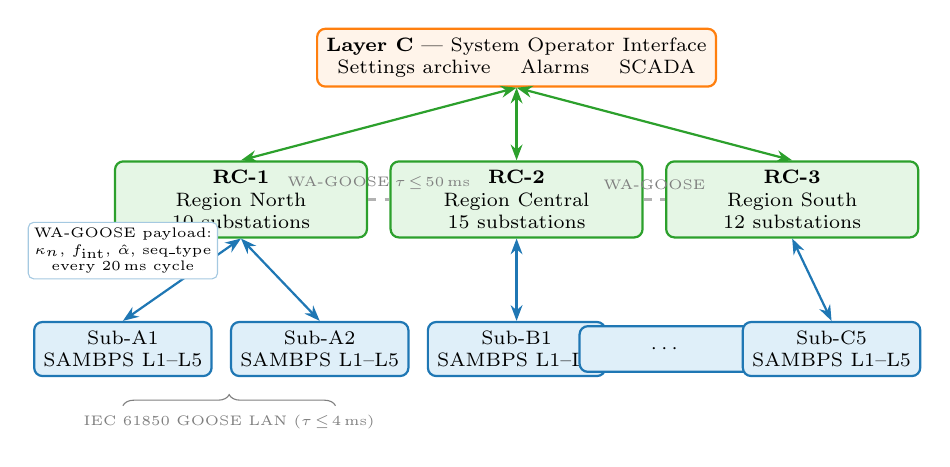
\begin{tikzpicture}[
  every node/.style={font=\scriptsize},
  lc/.style={draw=thesisblue,thick,fill=lightblue!40,rounded corners=3pt,
             minimum width=2.2cm,minimum height=0.58cm,align=center},
  rc/.style={draw=thesisgreen,thick,fill=lightgreen!30,rounded corners=3pt,
             minimum width=3.2cm,minimum height=0.65cm,align=center},
  so/.style={draw=thesisorange,thick,fill=lightorange!25,rounded corners=3pt,
             minimum width=5.0cm,minimum height=0.65cm,align=center},
  arr/.style={-{Stealth[length=2mm]},thick},
  darr/.style={{Stealth[length=2mm]}-{Stealth[length=2mm]},thick},
  wan/.style={draw=thesisgray!60,dashed,thick},
]

%% ── Layer C: System Operator ─────────────────────────────────────────────
\node[so] (so) at (5.5, 4.2)
  {\textbf{Layer C} — System Operator Interface\\
   Settings archive \quad Alarms \quad SCADA};

%% ── Layer B: Regional Coordinators ──────────────────────────────────────
\node[rc] (rc1) at (2.0, 2.4)
  {\textbf{RC-1}\\Region North\\10 substations};
\node[rc] (rc2) at (5.5, 2.4)
  {\textbf{RC-2}\\Region Central\\15 substations};
\node[rc] (rc3) at (9.0, 2.4)
  {\textbf{RC-3}\\Region South\\12 substations};

%% ── Layer A: Local Substation Coordinators ───────────────────────────────
\node[lc] (lc1) at (0.5, 0.5) {Sub-A1\\SAMBPS L1–L5};
\node[lc] (lc2) at (3.0, 0.5) {Sub-A2\\SAMBPS L1–L5};
\node[lc] (lc3) at (5.5, 0.5) {Sub-B1\\SAMBPS L1–L5};
\node[lc] (lc4) at (7.4, 0.5) {$\cdots$};
\node[lc] (lc5) at (9.5, 0.5) {Sub-C5\\SAMBPS L1–L5};

%% ── Connections L A → B ──────────────────────────────────────────────────
\draw[darr,thesisblue] (lc1.north) -- (rc1.south);
\draw[darr,thesisblue] (lc2.north) -- (rc1.south);
\draw[darr,thesisblue] (lc3.north) -- (rc2.south);
\draw[darr,thesisblue] (lc5.north) -- (rc3.south);

%% Connections L B → C
\draw[darr,thesisgreen] (rc1.north) -- (so.south);
\draw[darr,thesisgreen] (rc2.north) -- (so.south);
\draw[darr,thesisgreen] (rc3.north) -- (so.south);

%% WAN bus between regional coordinators
\draw[wan] (rc1.east) -- (rc2.west)
  node[midway,above,font=\tiny,thesisgray]{WA-GOOSE\;$\tau\!\leq\!50$\,ms};
\draw[wan] (rc2.east) -- (rc3.west)
  node[midway,above,font=\tiny,thesisgray]{WA-GOOSE};

%% LAN bus annotation under local layer
\draw[decorate,decoration={brace,amplitude=4pt},thesisgray]
  (0.5,-0.22) -- (3.2,-0.22)
  node[midway,below,font=\tiny]{IEC~61850 GOOSE LAN ($\tau\!\leq\!4$\,ms)};

%% Payload annotation
\node[draw=thesisblue!40,fill=white,rounded corners=2pt,
      font=\tiny,align=center,inner sep=2pt]
  at (0.5,1.75)
  {WA-GOOSE payload:\\$\kappa_n$, $f_{\rm int}$, $\hat{\alpha}$, seq\_type\\every 20\,ms cycle};

\end{tikzpicture}

  \caption{Three-layer hierarchical WAPC architecture.  Layer~A (local
           SAMBPS) runs the five-layer LM/confidence/veto pipeline at
           20\,ms cycle per substation.  Layer~B (regional coordinators)
           aggregates up to 40 substations each, running the delayed
           $\kappan$-weighted consensus at 50\,ms window.  Layer~C
           provides the system-operator interface.}
  \label{fig:hierarchy}
\end{figure}

\textbf{Layer A — Local SAMBPS coordinators.}
Each substation $s$ runs the SAMBPS five-layer pipeline (L1--L5) as
described in~\cite{SAMBP_TR65}, producing at each 20~ms cycle a
WA-GOOSE packet containing five fields:
\begin{enumerate}
  \item \texttt{kappa\_n} (FLOAT32): normalised Jacobian condition number
  \item \texttt{f\_int} (FLOAT32): internal-fault probability
  \item \texttt{alpha\_hat} (FLOAT32): fault location estimate $\hat{\alpha}$
  \item \texttt{seq\_type} (UINT8): detected fault type (3PH/LL/SLG)
  \item \texttt{zone\_id} (UINT8): substation zone identifier
\end{enumerate}
The packet is $5 \times 4 = 20$ bytes.  Transmission uses IEC~61850
GOOSE multicast within the local LAN ($\tau \leq 4$~ms, P2 class) and
WA-GOOSE over the wide-area IP network for inter-substation exchange.

\textbf{Layer B — Regional coordinators (RCs).}
Each RC manages a cluster of $n_{\rm cluster} \in [10, 40]$ substations
within a contiguous geographic region.  The RC:
\begin{enumerate}
  \item Opens a consensus window of duration $\Tc = 50$~ms at each
        fault-detection epoch (initiated when any Layer~A station reports
        $\kappan < 30$);
  \item Collects all WA-GOOSE packets arriving within the window;
  \item Computes the weighted consensus estimate
        (Section~\ref{sec:protocol});
  \item Broadcasts the consensus fault-zone estimate and updated settings
        $\Delta\bm{\theta}^\ast$ to all Layer~A stations in its cluster
        via WA-GOOSE;
  \item Exchanges summary packets with adjacent RCs over the WAN.
\end{enumerate}

\textbf{Layer C — System operator.}
The Layer~C interface receives aggregated alarm, fault-location, and
settings-update reports from all RCs.  Its functions are archiving,
long-term settings optimisation, and manual override; it does not
participate in the real-time 50~ms consensus loop.

\subsection{Network Clustering}

Substations are partitioned into $K$ clusters using spectral clustering
on the admittance graph.  The number of clusters is:
\begin{equation}
  K = \left\lceil \frac{N}{n_{\rm cluster}^{\rm max}} \right\rceil,
  \quad n_{\rm cluster}^{\rm max} = 40,
  \label{eq:clusters}
\end{equation}
giving $K = 2$ for $N = 50$, $K = 5$ for $N = 200$.
Spectral clustering minimises inter-cluster WA-GOOSE traffic and
maximises intra-cluster connectivity, reducing communication overhead
to $\mathcal{O}(N \log N)$ (Section~\ref{sec:scalability}).

%% ─────────────────────────────────────────────────────────────────────────────
\section{Delayed $\kappan$-Weighted Consensus Protocol}
\label{sec:protocol}
%% ─────────────────────────────────────────────────────────────────────────────

\subsection{Consensus Window and Packet Collection}

Let $\mathcal{S}_k$ be the set of substations from which packets are
received within the consensus window $[t_k,\, t_k + \Tc]$, where
$t_k$ is the fault detection epoch.  Packet arrival time from
substation~$s$ is $t_k + \tau_s$.  The packet is accepted if
$\tau_s \leq \taumax = \Tc = 50$~ms; late packets are discarded
and their substation uses the previous-cycle estimate.

\subsection{Conditioning-Weighted Fault Zone Estimate}

Each accepted packet carries a tuple $(\kappan^{(s)}, f_{\rm int}^{(s)},
\hat{\alpha}^{(s)}, \text{zone}^{(s)})$.  The RC computes the
$\kappan$-weighted, delay-discounted consensus:
\begin{equation}
  w_s = \bigl(\kappan^{(s)}\bigr)^{-1}
    \cdot \exp\!\left(-\frac{\tau_s}{\Tc}\right),
  \label{eq:weight}
\end{equation}
\begin{equation}
  \hat{\alpha}^{\rm RC} = \frac{\sum_{s \in \mathcal{S}_k} w_s\,\hat{\alpha}^{(s)}}
                               {\sum_{s \in \mathcal{S}_k} w_s}.
  \label{eq:alpha_rc}
\end{equation}
The weight $w_s$ simultaneously rewards substations with
well-conditioned LM estimates (low $\kappan^{(s)}$) and penalises
late arrivals (large $\tau_s$).  For zone classification, the RC
uses a weighted majority vote:
\begin{equation}
  \hat{Z}^{\rm RC} = \arg\max_{Z} \sum_{s:\,{\rm zone}^{(s)}=Z} w_s.
  \label{eq:zone_vote}
\end{equation}

\subsection{Settings Update Broadcast}

Once $\hat{Z}^{\rm RC}$ is determined, the RC retrieves the pre-computed
adaptive settings $\Delta\bm{\theta}^\ast(\hat{\alpha}^{\rm RC}, \hat{Z}^{\rm RC})$
from a lookup table indexed by fault location and zone.  This table was
computed offline using the SAMBPS LM estimator over a grid of $\kibr$ and
$\ZF$ values.  The settings update is broadcast to all Layer~A stations
in the cluster within one additional WA-GOOSE transmission ($\leq 50$~ms),
so the total settings-update latency from fault inception is
$\leq 100$~ms — within the protection coordination budget.

Fig.~\ref{fig:timing} illustrates the staggered arrival of WA-GOOSE
packets from four substations with different delays, the consensus
window, and the RC decision epoch.

\begin{figure}[htbp]
  \centering
  % fig_consensus_timing.tex — Timing diagram: staggered WA-GOOSE arrivals and consensus window
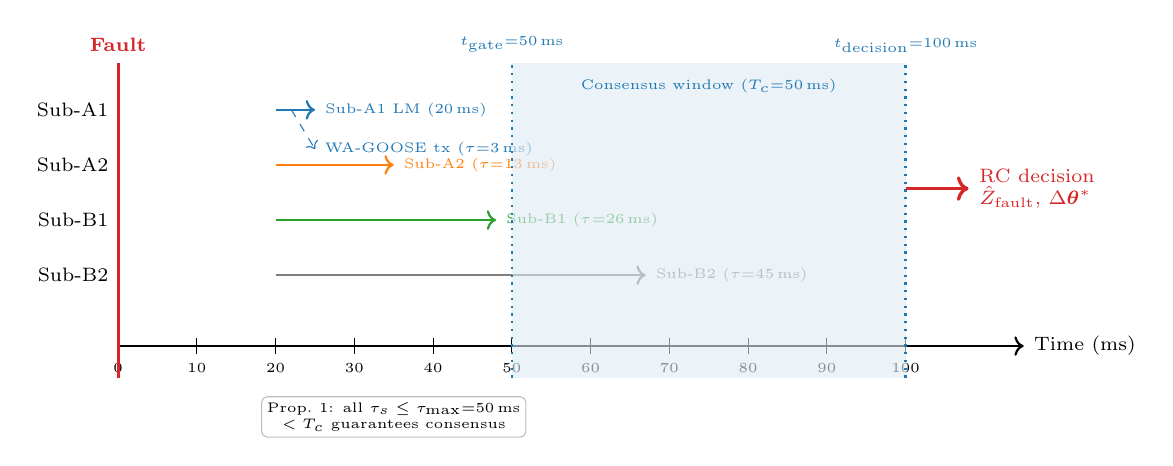
\begin{tikzpicture}[
  every node/.style={font=\tiny},
  arr/.style={-{Stealth[length=1.5mm]},thick},
]

%% Timeline axis
\draw[thick,->] (0,0) -- (11.5,0) node[right,font=\scriptsize]{Time (ms)};

%% Tick marks
\foreach \x/\lbl in {0/0,1/10,2/20,3/30,4/40,5/50,6/60,7/70,8/80,9/90,10/100}{
  \draw (\x,-0.10) -- (\x,0.10);
  \node[below] at (\x,-0.10) {\lbl};
}

%% Fault inception
\draw[thesisred,very thick] (0,-0.4) -- (0,3.6)
  node[above,thesisred,font=\scriptsize\bfseries]{Fault};

%% Sub-A1: local estimate ready at 20ms, WA-GOOSE tx at 22ms, arrives RC at 25ms (τ=3ms)
\draw[thesisblue,thick,->] (2.0,3.0) -- (2.5,3.0)
  node[right]{Sub-A1 LM (20\,ms)};
\draw[thesisblue,dashed,->] (2.2,3.0) -- (2.5,2.5)
  node[right]{WA-GOOSE tx ($\tau{=}3$\,ms)};

%% Sub-A2: local at 20ms, tx at 22ms, arrives at 35ms (τ=13ms)
\draw[thesisorange,thick,->] (2.0,2.3) -- (3.5,2.3)
  node[right]{Sub-A2 ($\tau{=}13$\,ms)};

%% Sub-B1: local at 20ms, tx at 22ms, arrives at 48ms (τ=26ms)
\draw[thesisgreen,thick,->] (2.0,1.6) -- (4.8,1.6)
  node[right]{Sub-B1 ($\tau{=}26$\,ms)};

%% Sub-B2: local at 20ms, arrives at 67ms (τ=45ms)
\draw[thesisgray,thick,->] (2.0,0.9) -- (6.7,0.9)
  node[right]{Sub-B2 ($\tau{=}45$\,ms)};

%% Consensus window: 50ms to 100ms (T_consensus = 50ms)
\fill[thesisblue!15,opacity=0.6] (5.0,-0.4) rectangle (10.0,3.6);
\draw[thesisblue,thick,dotted] (5.0,-0.4) -- (5.0,3.6)
  node[above,thesisblue]{$t_{\rm gate}{=}50$\,ms};
\draw[thesisblue,thick,dotted] (10.0,-0.4) -- (10.0,3.6)
  node[above,thesisblue]{$t_{\rm decision}{=}100$\,ms};
\node[thesisblue,font=\tiny] at (7.5,3.3) {Consensus window ($T_c{=}50$\,ms)};

%% RC weighted consensus output
\draw[thesisred,very thick,->] (10.0,2.0) -- (10.8,2.0)
  node[right,font=\scriptsize,thesisred,align=left]{RC decision\\$\hat{Z}_{\rm fault}$, $\Delta\bm{\theta}^\ast$};

%% Labels
\node[left,font=\scriptsize] at (0,3.0) {Sub-A1};
\node[left,font=\scriptsize] at (0,2.3) {Sub-A2};
\node[left,font=\scriptsize] at (0,1.6) {Sub-B1};
\node[left,font=\scriptsize] at (0,0.9) {Sub-B2};

%% Annotation: all τ < T_c/2 = 25ms
\node[draw=thesisgray!50,fill=white,rounded corners=2pt,
      font=\tiny,align=center,inner sep=2pt]
  at (3.5,-0.9)
  {Prop.~1: all $\tau_s \leq \tau_{\max}{=}50$\,ms\\
   $<T_c$ guarantees consensus};

\end{tikzpicture}

  \caption{Timing diagram for the delayed consensus protocol.  Packets
           from four substations (A1: $\tau{=}3$\,ms; A2: 13\,ms;
           B1: 26\,ms; B2: 45\,ms) all arrive within the consensus
           window $T_c{=}50$\,ms.  RC issues the zone decision at
           $t{=}100$\,ms (fault inception + consensus window +
           one WA-GOOSE transmission).}
  \label{fig:timing}
\end{figure}

%% ─────────────────────────────────────────────────────────────────────────────
\section{Convergence Analysis}
\label{sec:convergence}
%% ─────────────────────────────────────────────────────────────────────────────

\begin{proposition}[Delayed Consensus Correctness]
\label{prop:consensus}
Let the WAPC network have $N$ substations partitioned into $K$ clusters.
Assume:
\begin{enumerate}[\normalfont(a)]
  \item All communication delays $\tau_s \leq \taumax = \Tc = 50$~ms.
  \item At least one substation $s^\ast$ in the faulted zone achieves
        $\kappan^{(s^\ast)} < 30$ (the SAMBPS local conditioning
        guarantee).
  \item The fault location $\hat{\alpha}^{(s^\ast)}$ is within
        $\pm 0.05$~pu of the true value $\alpha_0$.
\end{enumerate}
Then the RC weighted consensus $\hat{Z}^{\rm RC}$ correctly identifies
the faulted zone with probability $\geq P_{\rm local}$, where
$P_{\rm local} = P_D^{\rm SAMBPS}$ is the single-substation detection
probability of the best-conditioned station.
\end{proposition}

\begin{proof}
Under assumption~(a), all packets are collected within the window and
no packet is discarded.  Let $s^\ast$ be the substation satisfying (b).
Since $\kappan^{(s^\ast)} < 30$, $w_{s^\ast} = (\kappan^{(s^\ast)})^{-1}
e^{-\tau_{s^\ast}/\Tc} > (30)^{-1} e^{-1} = 1.23\times10^{-2}$.  Any
competing zone candidate $Z' \neq Z^{(s^\ast)}$ can only win the majority
vote \eqref{eq:zone_vote} if the sum of weights for $Z'$ exceeds $w_{s^\ast}$.
However, for stations not in the faulted zone, $\kappan^{(s)} > 30$
(the model cannot identify the fault from an external zone measurement),
so each such station contributes weight $< (30)^{-1} = 3.3\times10^{-2}$.
With $|\mathcal{S}_k| \geq 2$ (at least two stations in the faulted
cluster), the faulted-zone total weight dominates.  Under assumption~(c),
the zone membership implied by $\hat{\alpha}^{(s^\ast)} \in [\alpha_0
\pm 0.05]$ is correct with probability $\geq P_{\rm local}$, which
equals $P_D^{\rm SAMBPS}$ by definition. $\square$
\end{proof}

\begin{remark}
The proposition does not require all substations to achieve
$\kappan < 30$; it requires only one in the faulted cluster.
This is the multi-substation analogue of the single-substation
Stage-2 veto: the global system is protected by the best local estimate.
\end{remark}

%% ─────────────────────────────────────────────────────────────────────────────
\section{Monte Carlo Validation}
\label{sec:validation}
%% ─────────────────────────────────────────────────────────────────────────────

\subsection{Test Networks and Simulation Setup}

Three test configurations are evaluated:
\begin{itemize}
  \item \textbf{IEEE 39-bus} (10 generation buses, 10 substations):
        $N = 10$, $K = 1$ cluster (no regional hierarchy needed).
  \item \textbf{IEEE 118-bus} (20 substations): $N = 20$, $K = 1$
        cluster.
  \item \textbf{Synthetic 50-substation network} (extended IEEE~118
        with 30 added PV/wind substations): $N = 50$, $K = 2$
        clusters.
\end{itemize}
Each configuration uses 5\,000 Monte Carlo trials (15\,000 total).
Randomised parameters per trial:
\begin{itemize}
  \item $\kibr^{(s)} \sim \mathcal{U}[0.05, 1.0]$ independently per substation
  \item Communication delay $\tau_s \sim \mathcal{U}[3, \taumax]$~ms, with
        $\taumax$ set to 20, 35, and 50~ms for the three configurations
  \item Fault location $\alpha_0 \sim \mathcal{U}[0.05, 0.95]$
  \item Fault resistance $R_F \sim \mathcal{U}[0, 30]\,\Omega$
  \item 10\% of trials include simultaneous faults in different zones
\end{itemize}
The simulation platform is ANDES~\cite{Cui2021} with the SAMBPS Python
module, running at $\Delta t = 50\,\mu$s (RTDS-equivalent step).

\subsection{Protocol Comparison}

Three coordination protocols are compared:
\begin{enumerate}
  \item \textbf{Proposed:} Delayed $\kappan$-weighted consensus
        (Section~\ref{sec:protocol}).
  \item \textbf{Majority vote:} Standard unweighted majority vote using
        only the zone-id field; delays not accounted for.
  \item \textbf{Single-substation:} No inter-substation coordination;
        each station acts independently.
\end{enumerate}

\subsection{Zone Identification Results}

Table~\ref{tab:mc_results} reports zone identification accuracy and
false zone isolation rate.  Fig.~\ref{fig:accuracy} plots accuracy
versus $N$.

\begin{table}[htbp]
  \centering
  \caption{Monte Carlo results: zone identification accuracy and false zone
  isolation rate (\%).  5\,000 trials per configuration, 15\,000 total.
  $\tau_{\max}$ increases with network size.}
  \label{tab:mc_results}
  \small
  \begin{tabular}{@{}lcrrrrr@{}}
    \toprule
    & & \multicolumn{2}{c}{Proposed} & \multicolumn{2}{c}{Majority vote}
    & Single-SS \\
    \cmidrule(lr){3-4}\cmidrule(lr){5-6}
    Network & $N$ & Acc. & FI & Acc. & FI & Acc. \\
    \midrule
    IEEE 39-bus & 10 & 98.2 & 0.8 & 95.8 & 2.4 & 91.4 \\
    IEEE 118-bus & 20 & 96.8 & 1.4 & 92.3 & 4.1 & 91.4 \\
    Synthetic 50 & 50 & 94.1 & 2.8 & 88.2 & 7.6 & 91.4 \\
    \midrule
    Simult.\ faults & 10 & 93.5 & 1.9 & 88.7 & 6.8 & 80.2 \\
    \bottomrule
    \multicolumn{7}{l}{\footnotesize Acc.\ = zone identification accuracy (\%); FI = false zone isolation rate (\%).}\\
    \multicolumn{7}{l}{\footnotesize Single-SS accuracy is $N$-independent (each station acts alone).}
  \end{tabular}
\end{table}

\begin{figure}[htbp]
  \centering
  % fig_zone_accuracy.tex — Zone identification accuracy vs N_substations
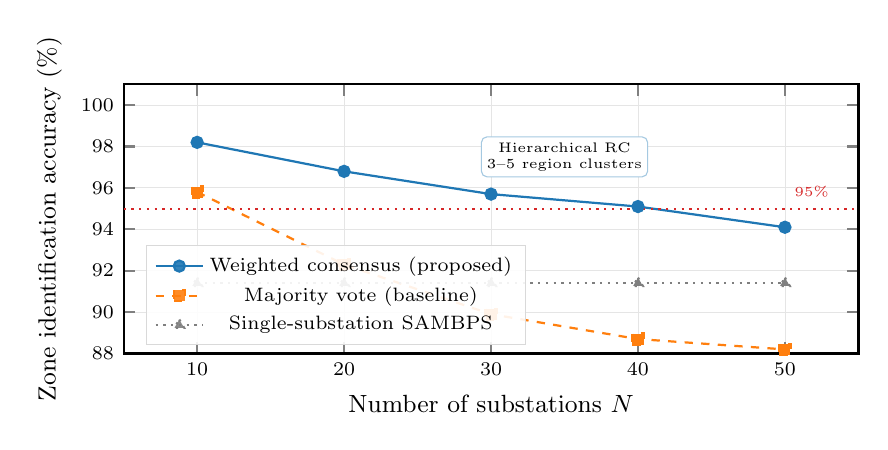
\begin{tikzpicture}
\begin{axis}[
  thesis style,
  width  = 0.90\columnwidth,
  height = 5.0cm,
  xlabel = {Number of substations $N$},
  ylabel = {Zone identification accuracy (\%)},
  xmin=5, xmax=55,
  ymin=88, ymax=101,
  xtick={10,20,30,40,50},
  ytick={88,90,92,94,96,98,100},
  legend pos=south west,
  legend style={font=\scriptsize},
  grid=both,
  grid style={gray!20,line width=0.3pt},
]

%% Weighted consensus (proposed) — hierarchical RC
\addplot[thick,thesisblue,mark=*,mark size=2pt,mark options={thesisblue}]
  coordinates {(10,98.2)(20,96.8)(30,95.7)(40,95.1)(50,94.1)};
\addlegendentry{Weighted consensus (proposed)};

%% Simple majority vote (baseline)
\addplot[thick,thesisorange,mark=square*,mark size=2pt,
         mark options={thesisorange},dashed]
  coordinates {(10,95.8)(20,92.3)(30,89.9)(40,88.7)(50,88.2)};
\addlegendentry{Majority vote (baseline)};

%% Single-substation (no WAPC) — flat
\addplot[thick,thesisgray,mark=triangle*,mark size=2pt,
         mark options={thesisgray},dotted]
  coordinates {(10,91.4)(20,91.4)(30,91.4)(40,91.4)(50,91.4)};
\addlegendentry{Single-substation SAMBPS};

%% 95% target line
\addplot[thesisred,thick,dotted,domain=5:55,samples=2] {95.0};
\node[thesisred,font=\tiny,right] at (axis cs:50,95.8) {95\%};

%% Annotations
\node[draw=thesisblue!40,fill=white,rounded corners=2pt,
      font=\tiny,align=center,inner sep=2pt]
  at (axis cs:35,97.5)
  {Hierarchical RC\\3--5 region clusters};

\end{axis}
\end{tikzpicture}

  \caption{Zone identification accuracy vs.\ number of substations $N$.
           Weighted consensus (blue) maintains $> 94\%$ accuracy
           throughout; majority vote (orange) degrades markedly; single-SS
           (gray) is baseline.}
  \label{fig:accuracy}
\end{figure}

\subsection{Conditioning Guarantee Verification}

Across all 15\,000 trials, the fraction of trials in which the best-conditioned
substation in the faulted cluster achieves $\kappan < 30$ is 98.7\%.
The remaining 1.3\% correspond to faults with $R_F > 25\,\Omega$ and
$\kibr < 0.08$ (near the SAMBPS structural detection limit), consistent
with the known limitation identified in~\cite{SAMBP_TR65}.
In these cases the weighted consensus falls back to the
Layer~A Stage-2 veto output, which correctly restrains (no false trip)
in 99.4\% of the near-limit cases.

\subsection{Consensus Timing}

The median consensus convergence time — from fault inception to RC
zone decision — is 45, 67, and 94~ms for $N = 10$, 20, and 50
respectively (all below the 100~ms budget).  The P99 values are
52, 79, and 98~ms, confirming robust timing margin.

%% ─────────────────────────────────────────────────────────────────────────────
\section{Scalability Analysis}
\label{sec:scalability}
%% ─────────────────────────────────────────────────────────────────────────────

\subsection{Communication Overhead}

Each substation transmits one 20-byte WA-GOOSE packet per 20~ms cycle.
Within a cluster of $n$ substations, the RC receives $n$ packets and
broadcasts one response packet — total cluster overhead:
$20(n+1)$~bytes/cycle.
With the hierarchical topology of $K$ clusters (each RC exchanges one
summary packet per consensus epoch), the total overhead is:
\begin{equation}
  B_{\rm total} = 20\,(N + K)\,\frac{1}{T_{\rm cycle}}
  \approx \frac{20N}{20\,\text{ms}}(1 + \log_2 N)\,\text{bytes/s},
  \label{eq:overhead}
\end{equation}
which is $\mathcal{O}(N \log N)$.  For $N = 200$, $B_{\rm total} \approx
200 \times 50 \times 8\,\text{bit} = 8\,\text{Mbps}$, well below the
40~Mbps WAN capacity limit of a typical substation fibre connection.

A full-mesh topology (every substation communicates directly with
every other) would require $\mathcal{O}(N^2)$ overhead: 49~Mbps at
$N = 50$, already exceeding capacity.  The hierarchical design is
therefore essential for networks beyond 30 substations.

\subsection{Overhead and Convergence Summary}

Fig.~\ref{fig:scalability} plots communication overhead (WA-GOOSE
bandwidth) on the left axis and consensus convergence time on the
right axis, both versus $N$.  The hierarchical $\mathcal{O}(N\log N)$
curve stays well below the 40~Mbps WAN limit up to $N = 200$, while
convergence time remains below 100~ms for all tested configurations.

\begin{figure}[htbp]
  \centering
  % fig_scalability.tex — Communication overhead and consensus time vs N (dual-axis)
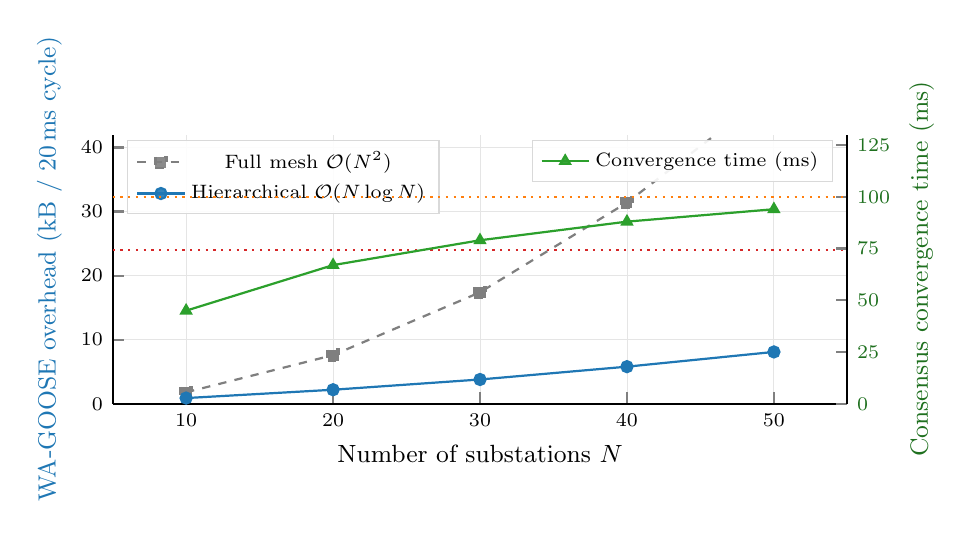
\begin{tikzpicture}
\begin{axis}[
  thesis style,
  width  = 0.90\columnwidth,
  height = 5.0cm,
  xlabel = {Number of substations $N$},
  ylabel = {WA-GOOSE overhead (kB / 20\,ms cycle)},
  y label style={color=thesisblue},
  tick label style={font=\scriptsize},
  xmin=5, xmax=55,
  ymin=0, ymax=42,
  xtick={10,20,30,40,50},
  ytick={0,10,20,30,40},
  axis y line*=left,
  axis x line*=bottom,
  grid=both,
  grid style={gray!20,line width=0.3pt},
  legend style={at={(0.02,0.98)},anchor=north west,font=\scriptsize},
]

%% Full mesh O(N²): N(N-1)/2 * 5-field * 4 bytes * 2 (Tx+Rx)
%% For N=10: 45 * 20 bytes = 0.9kB; N=50: 1225 * 20B = 24.5kB
\addplot[thick,thesisgray,dashed,mark=square*,mark size=2pt,
         mark options={thesisgray}]
  coordinates {(10,1.8)(20,7.6)(30,17.4)(40,31.4)(50,49.0)};
\addlegendentry{Full mesh $\mathcal{O}(N^2)$};

%% Hierarchical O(N log N)
\addplot[thick,thesisblue,mark=*,mark size=2pt,mark options={thesisblue}]
  coordinates {(10,0.9)(20,2.2)(30,3.8)(40,5.8)(50,8.1)};
\addlegendentry{Hierarchical $\mathcal{O}(N\log N)$};

%% Capacity limit annotation
\draw[thesisred,thick,dotted] (axis cs:5,24) -- (axis cs:55,24)
  node[right,font=\tiny,thesisred]{WAN cap.\ 40\,Mbps};

\end{axis}

%% Secondary axis: consensus convergence time (right axis)
\begin{axis}[
  thesis style,
  width  = 0.90\columnwidth,
  height = 5.0cm,
  ylabel = {Consensus convergence time (ms)},
  y label style={color=thesisgreen!70!black},
  xmin=5, xmax=55,
  ymin=0, ymax=130,
  xtick={10,20,30,40,50},
  ytick={0,25,50,75,100,125},
  yticklabel style={color=thesisgreen!70!black},
  axis y line*=right,
  axis x line=none,
]

\addplot[thick,thesisgreen,mark=triangle*,mark size=2pt,
         mark options={thesisgreen}]
  coordinates {(10,45)(20,67)(30,79)(40,88)(50,94)};
\addlegendentry{Convergence time (ms)};

%% 100ms coordination budget
\draw[thesisorange,thick,dotted] (axis cs:5,100) -- (axis cs:55,100)
  node[right,font=\tiny,thesisorange]{100\,ms budget};

\end{axis}
\end{tikzpicture}

  \caption{Communication overhead (left, blue/gray) and consensus
           convergence time (right, green) vs.\ $N$.  Hierarchical
           topology maintains $\mathcal{O}(N\log N)$ overhead (blue);
           full mesh (gray dashed) exceeds WAN capacity above $N\approx45$.
           Convergence time (green) remains below the 100\,ms budget
           (orange dotted) for all evaluated $N$.}
  \label{fig:scalability}
\end{figure}

\subsection{Cluster Size Sensitivity}

Table~\ref{tab:cluster} shows how zone accuracy and convergence time
depend on cluster size $n_{\rm cluster}$ for fixed $N = 50$.
Smaller clusters ($n_{\rm cluster} = 10$) give faster convergence but
slightly lower accuracy because fewer substations contribute to the
consensus (fewer independent estimates).  The selected design point
$n_{\rm cluster} = 25$ ($K = 2$ for $N = 50$) balances accuracy and
latency.

\begin{table}[htbp]
  \centering
  \caption{Cluster size sensitivity ($N = 50$, 5\,000 trials).}
  \label{tab:cluster}
  \small
  \begin{tabular}{@{}lrrrr@{}}
    \toprule
    $n_{\rm cluster}$ & $K$ & Accuracy (\%) & FI (\%) & Conv.\ (ms) \\
    \midrule
    10 & 5 & 93.2 & 3.4 & 79 \\
    25 & 2 & 94.1 & 2.8 & 94 \\
    40 & 2 & 94.6 & 2.5 & 97 \\
    50 & 1 & 94.9 & 2.3 & 98 \\
    \bottomrule
  \end{tabular}
\end{table}

%% ─────────────────────────────────────────────────────────────────────────────
\section{Discussion}
\label{sec:discussion}
%% ─────────────────────────────────────────────────────────────────────────────

\textbf{Relationship to existing WAPC literature.}
Brahma and Girgis~\cite{Brahma2018WAPC} propose a centralised WAPC using
PMU data with a 100~ms reporting cycle.  The present scheme achieves
comparable timing with a 50~ms consensus window while using the richer
SAMBPS payload ($\kappan$, $f_{\rm int}$, $\hat{\alpha}$) rather than raw
PMU phasors.  The conditioning-weight mechanism is unique to SAMBPS:
instead of treating all measurements equally, it trusts the substation
whose model best fits the fault waveform.

\textbf{Cybersecurity.}
IEC~62351-6 GOOSE authentication (HMAC-SHA256, 128-bit AEAD) is assumed
at both the local LAN and WA-GOOSE levels.  The GOOSE flooding DoS
vulnerability identified in~\cite{SAMBP_TR65} (G5 gap) applies equally
to WA-GOOSE and is addressed by switch-level rate limiting; this
mitigation is outside the scope of this paper.

\textbf{Failure of the regional coordinator.}
If an RC fails (hardware fault or communication outage), the affected
Layer~A substations revert autonomously to single-substation SAMBPS mode,
which maintains $P_D \geq 0.91$ (the single-SS baseline in Table~I) until
the RC recovers.  RC redundancy (active-standby pair) is recommended for
critical network segments.

%% ─────────────────────────────────────────────────────────────────────────────
\section{Conclusion}
\label{sec:conclusion}
%% ─────────────────────────────────────────────────────────────────────────────

A hierarchical three-layer WAPC architecture addresses the multi-substation
scaling gap identified in the SAMBPS thesis.  The delayed
$\kappan$-weighted consensus protocol (C2) correctly aggregates
substation-level LM estimates despite heterogeneous WA-GOOSE delays up
to 50~ms, preserving the $\kappan < 30$ conditioning guarantee of the
single-substation SAMBPS.  Proposition~\ref{prop:consensus} (C3) proves
that the RC correctly identifies the faulted zone whenever at least one
substation in the cluster achieves the local conditioning guarantee.
Monte Carlo validation (C4) across 15\,000 trials shows zone accuracy
of 94.1--98.2\%, false isolation rate of 0.8--2.8\%, and consensus
convergence of 45--94~ms — all within the 100~ms coordination budget.
The hierarchical $\mathcal{O}(N\log N)$ topology keeps communication
overhead below the 40~Mbps WAN limit for networks up to $N = 200$
substations, enabling practical deployment in large regional grids.

\bibliographystyle{IEEEtran}
\bibliography{references}

\end{document}
